%%
%% This is file `example/ch_concln.tex',
%% generated with the docstrip utility.
%%
%% The original source files were:
%%
%% install/buptgraduatethesis.dtx  (with options: `ch-concln')
%% 
%% This file is a part of the example of BUPTGraduateThesis.
%% 

\chapter{相关技术概述}
SDN作为新一代的网络架构,具有动态配置、可编程及快速响应的特点,通过解耦控制平面与数据转发平面,实现了对网络底层基础设施的抽象。OpenStack是当下最流行的开源云平台,为用户提供计算、存储、网络服务。本章对SDN、OpenFlow、OpenStack等相关技术做了详细的介绍。
\section{SDN、OpenFlow概述}
\subsection{SDN简介}
SDN是一种时下热门的网络架构,在这种网络架构中,网络的控制与转发解耦,具有很强的可编程行和可扩展性。传统模式下,网络的控制权与网络设备紧密捆绑,现有模式下,控制权的迁移使得底层构架能够抽象出来,各种应用和网络服务因此能将网络当作一个逻辑或虚拟实体。通过应用SDN,网络的设计和操作变得简化,网络设备也得到简化,这些设备无需理解或处理成千上万的协议,只需要接受SDN控制器的指令即可。利用控制集中,网络管理员可以实时改变网络的行为,并且在几小时或几天内就可以部署新的应用和网络服务。

\begin{figure}[!htb]
  \centering
  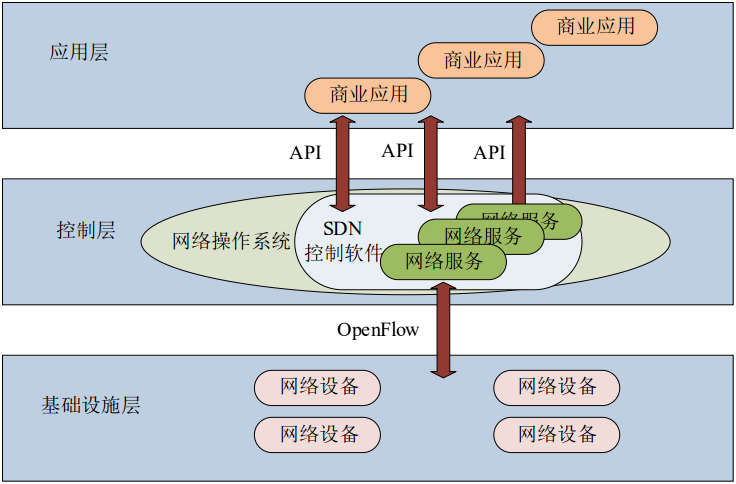
\includegraphics[width=0.7\textwidth]{logo/sdn.png}
  \caption{ONF定义的SDN三层架构图}
  \label{fig:sdn}
\end{figure}

传统网络设备紧耦合的构架在SDN体系中被拆分成应用、控制、转发三层分离的,可编程的开放构架。控制功能被转移到服务器(软件),上层应用、底层转发设施被抽象成多个逻辑实体。图\ref{fig:sdn}为ONF定义的SDN三层架构示意图。

应用层为网络各种应用需求,如移动视频、云存储、企业应用商店、桌面云、物联网等,通过北向接口灵活、可编程地调用控制层提供的网络抽象模型与业务功能。北向接口因为涉及业务较多,开放的标准化过程还处于研究阶段。

控制层为整个SDN构架的核心,也称为网络操作系统,可实现网络拓扑的集中控制和设备管理,进行流表的控制和下发。其主要功能包括路由优化、网络虚拟化、质量监控、拓扑管理、设备管理、接口适配等。

基础设施层包括标准化的网络设备和虚拟的网络设备,负责多级流表处理和高性能的数据转发,并作为硬件资源池,为控制层提供按需的网络拓扑、数据处理和数据转发。目前主流的网络设备和芯片产商已经提供了支持OpenFlow的网络设备。

南向接口定义了控制层与数据转发层(基础设施层)之间的交互协议,通过将转发过程抽象为流表,控制器可直接控制流表、屏蔽硬件,实现了网络虚拟化。物理硬件被淡化为资源池,可按需进行灵活分配和相互隔离。目前主流的控制层与转发层之间交互的协议为OpenFlow协议。
\subsection{OpenFlow协议}
OpenFlow协议是OpenFlow交换机和控制器之间交互信息的标准,也是OpenFlow交换机和控制器之间的接口标准。OpenFlow协议主要支持三种类型的消息:Controller-to-Switch消息,Asynchronous 消息和 Symmetric 消息。每种类型消息都有多个子类型。Controller-to-Switch消息由控制器发起直接管理和监视交换机状态,可能需要交换机做出响应;Asynchronous消息由交换机发起用于更新交换机的状态和控制器的网络事件;Symmetric消息可由控制器和交换机任一方发起。具体协议消息的类型及描述如下:

\begin{enumerate}
\item Controller-to-Switch消息
\begin{itemize}
\item Features:在建立传输层安全会话(Transport Layer Security Session)的时候,控制器发送feature请求消息给交换机,交换机需要应答自身支持的功能。一般在 OpenFlow 通道建立时使用。
\item Configuration:控制器设置或查询交换机上的配置信息。交换机仅需要应答查询消息。
\item Modify-state:控制器管理交换机流表项和端口状态等。
\item Read-state:控制器发送该消息来管理交换机状态。主要用于增加、删除或改变组/流表项和设置交换机端口属性。
\item Packet-out:控制器通过交换机指定端口发出网包。控制器按指定交换机端口发送数据包,并且转发经由Packet-in消息接收到的包。Packet-out消息必须包含完整包或一个指向存储在交换机中的完整包的缓冲区ID。该消息包含一系列按指定顺序执行的行为,若为空则丢弃该包。 
\item Barrier:控制器确保消息依赖满足,或接收完成操作的通知
\end{itemize}
\item Asynchronous消息
\begin{itemize}
\item Packet-in:交换机收到一个网包,在流表中没有匹配项,则发送Packet-in 消息给控制器。如果交换机缓存足够多,网包被临时放在缓存中,网包的部分内容(默认128 字节)和在交换机缓存中的的序号也一同发给控制器;如果交换机缓存不足以存储网包,则将整个网包作为消息的附带内容发给控制器。
\item Flow-removed:交换机中的流表项因为超时或修改等原因被删除掉,会触发Flow-removed 消息,通知控制器删除流表。
\item Port-status:交换机端口状态发生变化时(例如down 掉),触发Port-status 消息。
\item Error:交换机发生问题时触发消息。
\end{itemize}
\item Symmetric消息
\begin{itemize}
\item Hello:交换机和控制器用来建立连接。
\item Echo:交换机和控制器均可以向对方发出Echo消息,接收者则需要回复Echo reply。该消息用来测量延迟、带宽、以及是否连接正常等。
\item Vendor:交换机提供额外的附加信息功能。为未来版本预留。
\end{itemize}
\end{enumerate}

OpenFlow协议的主要交互过程如下所示:

\begin{enumerate}
\item 控制器与交换机的连接建立:通过安全通道建立连接,所有流量都不经过交换机流表检查。当连接建立起来后,两边必须先发送OFPT\_HELLO消息给对方,该消息携带支持的最高协议版本号,接收方将采用双方都支持的最低协议版本进行通信。一旦发现共同支持的协议版本,则连接建立,否则发送OFPT\_ERROR消息,描述失败原因,并中断连接。
\item 控制器与交换机的连接中断:当连接发生异常时,交换机应尝试连接备份的控制器。当多次尝试均失败后,交换机将进入紧急模式,并重置所有的TCP连接。此时,所有包将匹配指定的紧急模式表项,其他所有正常表项将从流表中删除。此外,当交换机刚启动时,默认进入紧急模式。
\item 连接加密:安全通道采用\gls*{TLS}连接加密。当交换机启动时,尝试连接到控制器的TCP 6633端口。双方通过交换证书进行认证。因此,每个交换机至少需配置两个证书,一个是用来认证控制器,一个用来向控制器发出认证。
\item 流表项修改:该交互是核心交互过程,通过控制器下发的流表项修改指令完成。每条指令可能触发一系列OpenFlow协议消息,主要包括流表的增加、修改和删除。
\item 流表项移除:流表项的移出包括控制器主动模式和被动模式,控制器被动模式下,定时器计时结束:每个表项均有一个idle\_timeout定时器和一个hard\_timeout定时器(两者的计量单位都是秒),前者计算的是没有Flow匹配发生的时间,而后者则计算的是表项在流表中的总时间。一旦到达时间期限,交换机将自动删除该表项,同时发出一个流删除的消息;控制器主动模式下,控制器通过下发DELETE\_STRICT、 DELETE等指令相关的协议消息主动删除流表项
\end{enumerate}

\subsection{OpenFlow交换机}
OpenFlow交换机负责数据转发功能,主要技术细节由流表(flow table)、安全信道(secure channel)组成\cite{openflow-1},如图\ref{fig:of-switch}所示。

\begin{figure}[!htb]
  \centering
  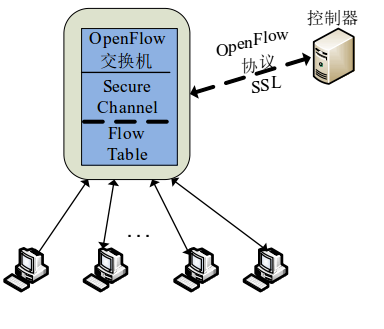
\includegraphics[width=0.7\textwidth]{logo/of-switch.png}
  \caption{OpenFlow交换机结构}
  \label{fig:of-switch}
\end{figure}

OpenFlow的转发策略主要保存在流表中,每个流表中都有很多表项(FlowEntry),这些表项可由外部控制器通过OpenFlow协议来写入、更新和删除。对于OpenFlow\ v1.3,每一个流表项都由匹配域、优先级、计数器、指令、超时以及Cookie组成,如表\ref{table:flow}所示。当一个流进入交换机后,交换机会选择匹配的流表中优先级最高的一个执行相应的指令并更新计数器、超时等项。

\newcommand{\enter}[2][c]{%
  \begin{tabular}[#1]{@{}c@{}}#2\end{tabular}}
\begin{table}[!htb]
    \centering
	\caption{OpenFlow流表项结构}
	\label{table:flow}
	\begin{tabular}{|c|c|c|c|c|c|}
	\hline 
	\enter{匹配域 \\(Match Field)}& \enter{优先级 \\(Priority)}& \enter{计数器 \\(Counters)}& \enter{指令\\(Instructions)}&\enter{超时 \\(Timeouts)} & Cookie \\
	\hline
	\end{tabular}
\end{table}

匹配域用于进行对流的匹配。包括13个必须支持的域(Required):入端口、Ethernet目的地址、源地址、类型、IP协议号、IPv4源地址、目的地址、IPv6源地址、目的地址、TCP源地址、目的地址、UDP源地扯、目的地址。每一个域包含一个确定的值或者任意值(Any,表示任何值都能匹配),更准确的匹配可以用位掩码实现,但是每个域对掩码的支持与否不同。

优先级用于在流匹配到多个表项时的选择策略,这里优先级最高的被优先匹配。

计数器用于维护每个流表、每个流、每个队列等的统计数据,例如活动表项、包查找次数、包匹配次数、发送包数、接收字节数等。指令执行于匹配到的包,每个表项包括一系列指令,这些指令可能会直接对包进行改变,也可能改变行动集,或者管道处理。其中行动集是在包被转发前按照指定顺序执行的一系列行动,管道处理是包在各流表之间进行传递时,包与流表之间的互相作用关系。

超时机制用于交换机对于超时表项的自动删除,进而提高交换机的空间利用率。包括硬超时(指超过该值即删除,绝对时间)和软超时(指超过该值也没有匹配的流即删除,相对时间)。

匹配的具体过程如图\ref{fig:match}所示,具体流程如下。

\begin{enumerate}
\item 数据匹配字段从数据包中提取。用于表查找的数据包匹配字段依赖与数据包类型,这些类型通常包括各种数据包的报头字段,如以太网源地址或IPv4目的地址。除了通过数据包报头中进行匹配,也可以通过入口端口和元数据字段进行匹配。元数据可以用来在一个交换机的不同表里面传递信息。报文匹配字段表示报文的当前状态,如果在前一个表中使用Apply-Actions改变了数据包的报头,那么这些变化也会在数据包匹配字段中反映。 
\item 数据包匹配字段中的值用于查找匹配的流表项。如果流表项字段具有该值,它就可以匹配包头中的所有可能的值。如果交换机支持任意的的位掩码对特定的匹配字段,这些掩码可以更精确地进行匹配。优先级最高的流表项首先被匹配上,此时与选择流表项相关的计数器也会被更新,选定流表项的指令集也被执行。如果有多个匹配的流表项具有相同的最高的优先级的,所选择的流表项被确定为未定义表项。
\end{enumerate}

\begin{figure}[!htb]
  \centering
  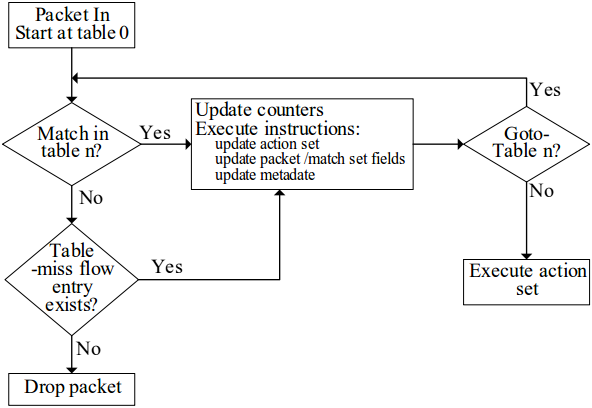
\includegraphics[width=0.7\textwidth]{logo/match.png}
  \caption{数据包匹配流程图}
  \label{fig:match}
\end{figure}

安全通道是连接OpenFlow交换机和控制器的接口,控制器通过这个接口,按照 OpenFlow协议规定的格式来配置和管理OpenFlow交换机,同时接收交换机传来的事件信息并发送数据包等。所有的OpenFlow通道信息必须用OpenFlow协议打包,OpenFlow通道通常用TLS来加密,但也能直接用TCP协议来实现。

目前,基于软件实现的 OpenFlow交换机主要有两个版本\cite{openflow-2},都部署于 Linux 系统:基于用户空间软件OpenFlow交换机操作简单,便于修改,但性能较差;基于内核空间的软件 OpenFlow 交换机\cite{openflow-3}速度较快,同时提供了虚拟化功能,使得每个虚拟机能够通过多个虚拟网卡传输流量,但实际的修改和操作过程较复杂。另外,斯坦福大学基于 NetFPGA 实现了硬件加速的线速 OpenFlow 交换机\cite{openflow-4},而网络硬件厂商如NEC、HP 等公司也已相继推出了支持 OpenFlow 标准的硬件交换机\cite{openflow-1}。
\subsection{OpenFlow控制器}
控制器是OpenFlow网络的核心部分,是整个网络的大脑,网络中所有的控制指令,数据流的转发操作都由它来完成,控制器中组件的好坏直接影响了整个网络的运行效率。


SDN控制器对网络的控制主要是通过南向接口协议实现,包括链路发现、拓扑管理、策略制定、表项下发等,其中链路发现和拓扑管理主要是控制其利用南向接口的上行通道对底层交换设备上报信息进行统一监控和统计,而策略制定和表项下发则是控制器利用南向接口的下行通道对网络设备进行统一控制。控制器负责控制其所管辖的OpenFlow交换机中的流表,包括流表内容的添加、修改以及删除等基本操作。操作的具体逻辑由控制器上运行的控制程序制定。网络使用者可以根据具体需求在控制器上编写控制程序,使得OpenFlow网络可以提供丰富的应用,体现了 OpenFlow网络的灵活性。在数据流处理的过程中,控制器的控制程序决定其所在网络中交换机上的流表内容。网路初始运行时,交换机上的流表为空,控制器必须具有全局网络视图, 如网络的拓扑结构、网络的当前运行状态等信息,才能针对不同数据流做出正确的决策。因此,控制器的设计是OpenFlow网络整体功能和效率的重点之一。

SDN北向接口是通过控制器向上层业务应用开放的接口,其目标是使得业务应用能够便利地调用底层的网络资源和能力。通过北向接口,网络业务的开发者能以软件编程的形式调用各种网络资源;同时上层的网络资源管理系统可以通过控制器的北向接口全局把控整个网网络的资源状态,并对资源进行统一调度。因为北向接口是直接为业务应用服务的,因此其设计需要密切联系业务应用需求具有多样化的特征。同时,北向接口的设计是否合理、便捷,以便能被业务应用广泛调用,会直接影响到SDN控制器厂商的市场前景。

控制器负责整个SDN网络的集中化控制,对于把握全网置资源视图、改善网络资源交付都具有非常重要的作用。但控制能力的集中化,也意味着控制器局的安全性和性能成为全网的瓶颈;另外,单一的控制器也无法应对跨多个地域的SND网络问题,需要多个SDN控制器组成的分布式集群,以避免单一的控制器节点在可靠性、扩展性、性能方面的问题。
\section{网络虚拟化技术概述}
互联网不断地向前发展,必然会出现越来越多的应用和服务。然而现有的网络结构比较僵化,而且可扩展性很差,随着网络的发展,这些缺点日益突出,但是研发和部署新型的网络体系架构比较因难,难以更新,而且由于各个设备生产商自身利益的考虑,更加加剧了这种困难。在这种背景下,网络虚拟化成为当前互联网面向未来网络体系架构过渡的一种有效解决方案,同时网络虚拟化也是未来网络体系架构应该具备的关键特性之一。

网络虚拟化技术\cite{Virtual-1},通过对共用的底层网络进行抽象并提供统一的可编程接口,将多个相互隔离且具有不同拓扑的虚拟网络映射到共用的基础设施上,为用户提供差异化服务。网络虚拟化允许多个租户占据相同的网络基础设施,每个租户会有一种错觉,认为可以对整个网络进行完整的处理.传统的网络虚拟化配置和操作都比较复杂,难以管理。原因就在于路由器和交换机变得越来越复杂,其配置操作的代价越来越大。而SDN的出现为网络虚拟化开启了另外一条道路,在SDN网络中,集中控制的优势使得对网络的管理变得灵活和高效。基于SDN的网络虚拟化是SDN思想的典型应用。本文选用OVX实现网络虚拟化模块,OVX通过给每个租户提供访问一个虚拟网络拓扑和一个完整的网络头空间来达到这样的目标,前者允许租户自定义拓扑结构,而后者保证功能性和流量隔离,即使是在不同的租户选择重叠的寻址方案。OVX用作控制信道内的一个代理,呈现OpenFlow网络给租户,同时经由南向的OpenFlow接口控制底层的物理基础设施。通过暴露OpenFlow网络给租户,OVX允许租户使用自己的网络控制器控制自有的虚拟网络资源。换句话说,OVX基于同一底层物理网络创建多个vSDN网络,并且vSDN网络之间是相互隔离的,保证了租户虚拟网络的安全性。这样的方法会产生两个后果:允许OVX呈现支持OpenFlow的可编程虚拟网络,租户可以使用自己的NOS控制虚拟网络,使OVX是透明的——从底层网络的角度,OVX的表现为一个控制器,从租户的角度上看,OVX作为网络中具有OpenFlow能力的交换机集合\cite{OVX-2}。OVX具体的架构图如图\ref{fig:ovx}所示。

\begin{figure}[!htb]
  \centering
  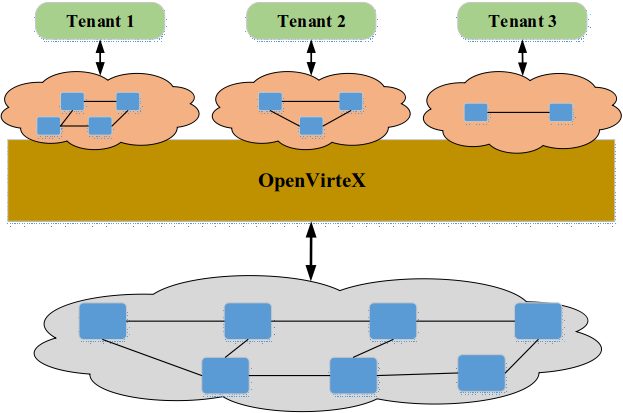
\includegraphics[width=0.7\textwidth]{logo/ovx.png}
  \caption{OVX网络虚拟化示意图}
  \label{fig:ovx}
\end{figure}

\section{OpenStack概述}

OpenStack是一个由NASA(美国国家航空航天局)和Rackspace合作研发并发起的,以Apache许可证授权的自由软件和开放源代码项目,主要为企业或者厂商提供了一种云服务的解决方案。OpenStack既可以被企业使用,在企业局域网内给员工提供私有云;也可以被厂商使用,进行二次开发,给云用户提供通过Internet访问的公有云服务。OpenStack通过一系列相关的服务提供IaaS解决方案。每个服务提供一个应用编程的API,这样有利于集成。管理员可以根据自己的需求安装部分或者全部服务。

\subsection{OpenStack架构}
OpenStack\ Juno版本的构架由9个服务组成,分别是Dashboard、Compute、Networking、Object Storage、Block Storage、Identity、Image Registry and Delivery Service、Telemetry和Orchestration。分别对应的各组件及各组件之间的协同关系如图\ref{fig:openstack}所示。

\begin{figure}[!htb]
  \centering
  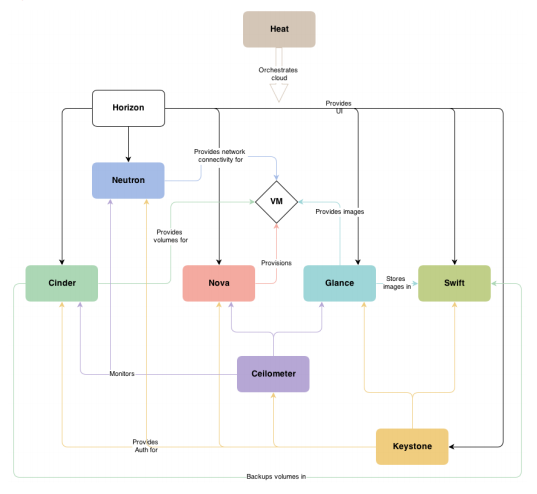
\includegraphics[width=0.7\textwidth]{logo/openstack.png}
  \caption{OpenStack概念架构图}
  \label{fig:openstack}
\end{figure}

主要组件的功能介绍如下\cite{OpenStack-3}。

\begin{enumerate}
\item Nova:计算服务是OpenStack的核心服务,它由nova-compute模块通过libvirt、XenAPI等管理hypervisor,从而管理虚拟机,此外它还通过nova-api服务向外提供如EC2兼容、管控功能等的接口,通过nova-scheduler模块提供虚拟机调研逻辑等,这些模块间的通信全部通过消息队列完成
\item Swift:对象存储服务是OpenStack最早期的两个服务之一(另一个是计算服务),在OpenStack平台中,任何的数据都是一个对象,swift-proxy模块对外提供如HTTP(S)、OpenStack Object API及与S3兼容的存取接口。对象的存取经swift-proxy接入后,还需要经三个模块进行定位,即account、container、object,这是因为在OpenStack中一个对象被描述为:某个帐户下某个容器中的某个对象。
\item Neutron:经过一定时间的演变,网络管理也抽离成一个独立的服务。在OpenStack的网络管理流程中,通常需要经过以下几个步骤:创建一个网络; 创建一个子网; 启动一个虚拟机,将一块网卡对接到指定的网络上;删除虚拟机;删除网络端口;删除网络。
\item Glance:Glance的出现是解决虚拟机镜像的管理问题,在生成一个镜像后,需要将镜像注册到系统的数据库中。当要实例化一个虚拟机时,需要将镜像分派到一台具体的实机上用来以启动虚拟机。因而Glance最重要的接口是镜像的注册和分派。
\item Cinder:Essex将nova的卷管理api独立化后,Folsom终于将卷管理服务抽离成了Cinder,Cinder管理所有的块存储设备,块设备可以挂接在虚拟机的实例中,然后虚拟机里的guest系统可以像操作本地卷一样操作块存储设备。Cinder需要处理的主要问题应该是接入各种块设备,如本地磁盘、LVM或各大广商提供的设备如EMC、NetApp、HP、华为,还有如Vmware提供的虚拟块设备等。
\item KeyStone:身份服务需要进行认证凭证的验证及关于用户、角色等的信息,及所有相关的元数据,这些数据全都由Keystone服务管理,并提供CRUD的操作方法,另外这些信息可以从另一个认证服务中获取,例如使用LDAP做Keystone的后端。
\item Heat:Heat是一套业务流程平台,旨在帮助用户更轻松地配置以OpenStack为基础的云体系。利用Heat应用程序,开发人员能够在程序中使用模板以实现资源的自动化部署。Heat能够启动应用、创建虚拟机并自动处理整个流程。
\item Ceilometer:Ceilometer项目创建时最初的目的是实现一个能为计费系统采集数据的框架。社区后来更新了他们的目标,新目标是希望Ceilometer成为OpenStack里数据采集(监控数据、计费数据)的唯一基础设施,采集到的数据提供给监控、计费、面板等项目使用。
\item Horizon:Horizon是一个用以管理、控制OpenStack服务的Web控制面板,它可以管理实例、镜像、创建密匙对,对实例添加卷、操作Swift容器等。除此之外,用户还可以在控制面板中使用终端(console)或VNC直接访问实例。
\end{enumerate}
\subsection{Neutron模块详解}
本文研究的主要内容,涉及最多的是OpenStack的Neutron模块,故本节对Neutron模块做详细的介绍,方便大家对论文的理解。

Neutron是OpenStack项目中负责提供网络服务的组件,它基于软件定义网络的思想,实现了网络虚拟化下的资源管理。在实现上充分利用了 Linux 系统上的各种网络相关的技术。一般的,OpenStack中网络实现包括VLAN、GRE、VXLAN等模式,本文中选取GRE模式搭建Neutron服务,GRE模式下的Neutron架构图如图\ref{fig:neutron}

\begin{figure}[!htb]
  \centering
  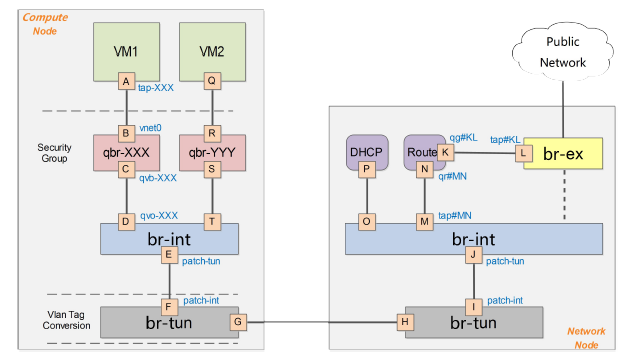
\includegraphics[width=0.7\textwidth]{logo/neutron.png}
  \caption{Neutron组件GRE模式架构图}
  \label{fig:neutron}
\end{figure}

在OpenStack中,所有网络有关的逻辑管理均在网络节点中实现,例如DNS、DHCP以及路由等。计算节点上只需要对所部属的虚拟机提供基本的网络功能支持,包括隔离不同租户的虚拟机和进行一些基本的安全策略管理(即安全组)。以抽象系统架构图为例,计算节点上包括两台虚拟机 VM1 和 VM2,分别经过一个网桥(如 qbr-XXX)连接到 br-int 网桥上。br-int 网桥再经过 br-tun 网桥(物理网络是 GRE 实现)连接到物理主机外部网络。网络节点上配置有DHCP、Router服务,对于访问外网的数据包,经由br-ex发出。各网桥功能及具体的服务如下所示。

\begin{enumerate}
\item qbr:在VM1中,虚拟机的网卡实际上连接到了物理机的一个TAP设(即 A常见名称如 tap-XXX)上,A 则进一步通过VETH pair(A-B)连接到网桥 qbr-XXX 的端口 vnet0(端口 B)上,之后再通过 VETH pair(C-D)连到br-int网桥上。一般C的名字格式为 qvb-XXX,而 D 的名字格式为 qvo-XXX。注意它们的名称除了前缀外,后面的id都是一样的,表示位于同一个虚拟机网络到物理机网络的连接上。之所以 TAP 设备 A 没有直接连接到网桥br-int上,是因为 OpenStack 需要通过iptables实现安全组的功能。目前 openvswitch 并不支持应用iptables 规则的 Tap 设备。因为 qbr 的存在主要是为了辅助 iptables 来实现 security group功能,有时候也被
称为 安全网桥 。
\item br-int:br-int是一个openvswitch网桥。br-int 在 GRE 模式中作为一个 NORMAL 交换机使用,因此有效规则只有一条正常转发。如果两个在同一主机上的 vm 属于同一个 tenant 的(同一个 vlan tag),则它们之间的通信只需要经过 br-int 即可。
\item br-tun:br-tun将带有 vlan tag 的 vm 跟外部通信的流量转换到对应的 gre 隧道,这上面要
实现主要的转换逻辑,规则要复杂,一般通过多张表来实现。这些规则组成的整体转发逻辑如图\ref{fig:br-tun}所示。

\begin{figure}[!htb]
  \centering
  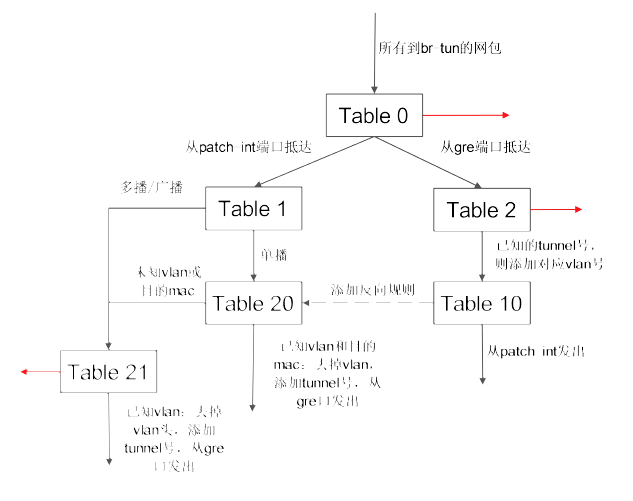
\includegraphics[width=0.7\textwidth]{logo/br-tun.png}
  \caption{br-tun网桥转发规则}
  \label{fig:br-tun}
\end{figure}

\item br-ex:br-ex直接连接到外部物理网络,一般情况下网关在物理网络中已经存在,则直接转发即可。
\item dhcp 服务:dhcp 服务是通过 dnsmasq 进程(轻量级服务器,可以提供 dns、dhcp、tftp 等服务)来实现的,该进程绑定到 dhcp 名字空间中的 br-int 的接口上。可以查看相关的进程。
\item router服务:首先,要理解什么是 router,router 是提供跨 subnet 的互联功能的。比如用户的内
部网络中主机想要访问外部互联网的地址,就需要 router 来转发(因此,所有跟外部网络的流量都必须经过 router)。目前 router 的实现是通过 iptables 进行的。 同样的,router 服务也运行在自己的名字空间中。防火墙服务就是在router命名空间中实现。

\end{enumerate}

\section{本章小结}
本章主要介绍了SDN、网络虚拟化及OpenStack的相关技术。重点介绍了OpenFlow协议,OpenFlow交换机的组成以及OpenFlow流表的字段和匹配过程。对于网络虚拟化技术,由于本文需要实现SDN模式下的网络虚拟化,所以仅对适用于本文的SDN模式下的网络虚拟化技术做了简单的概括。随后介绍了OpenStack的模块构成,而对于本文用到的Neutron模块,进行了详细的架构剖析。本研究的系统,主要在以上各部分的基础上,进行了集成开发。后续会对整体的系统架构做详细的介绍。